%%%%%%%%%%%%%%%%%%%%%%%%%%%%%%%%%%%%%%%%%%%%%%%%%%%%%%%%%%%%%%%%%%%%%%%%%%%%%%
%%%%%%%%%%%%%%%%%%%%%%%%%%%%%%%%%%%%%%%%%%%%%%%%%%%%%%%%%%%%%%%%%%%%%%%%%%%%%%
%%
%% Dokumentacia k projektu z IFJ
%% Autor: Martin Maga,Vit Mojzis, Viktor Malik, Vojtech Meca,Jiri Macku 
%% Datum: 27.11.2012
%%%%%%%%%%%%%%%%%%%%%%%%%%%%%%%%%%%%%%%%%%%%%%%%%%%%%%%%%%%%%%%%%%%%%%%%%%%%%%
%%%%%%%%%%%%%%%%%%%%%%%%%%%%%%%%%%%%%%%%%%%%%%%%%%%%%%%%%%%%%%%%%%%%%%%%%%%%%%
\documentclass[12pt,a4paper,titlepage,final]{article}
\newcommand{\uv}[1]{\quotedblbase #1\textquotedblleft}
% cestina a fonty
\usepackage[czech]{babel}
\usepackage[utf8]{inputenc}
% balicky pro odkazy
\usepackage[bookmarksopen,colorlinks,plainpages=false,urlcolor=blue,unicode]{hyperref}
\usepackage{url}
% obrazky
\usepackage[dvipdf]{graphicx}
% velikost stranky
\usepackage{graphicx}
\usepackage[top=3.5cm, left=2.5cm, text={17cm, 24cm}, ignorefoot]{geometry}

\begin{document}

\begin{titlepage}

\begin{figure}[h]
\begin{center}
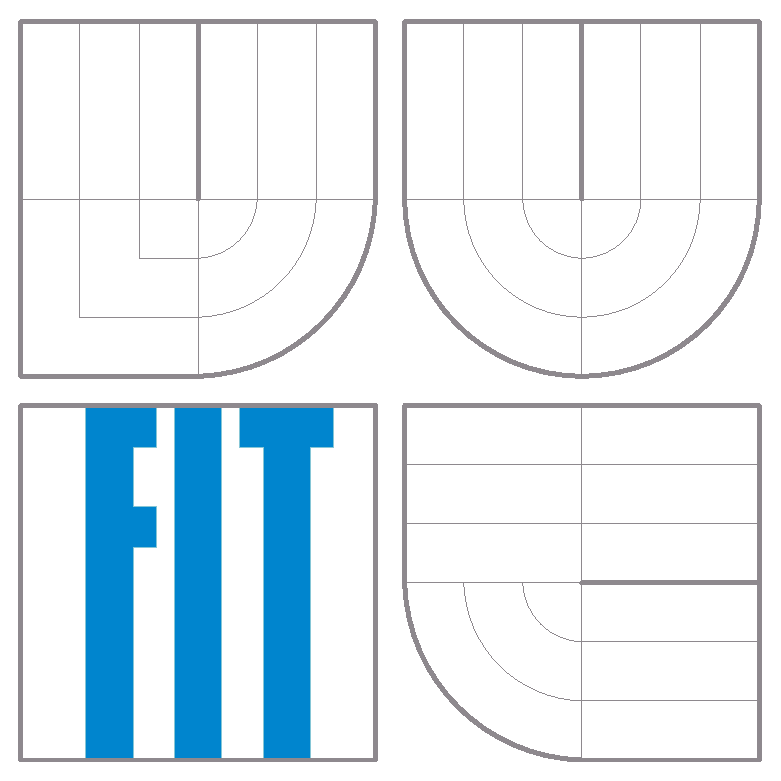
\includegraphics[scale=0.6]{logo.eps}
\end{center}
\end{figure}

\begin{center}
\LARGE
\textsc{Vysoké učení
  technické v~Brně\\ \Large{Fakulta informačních technológií}}\\
\vspace{\stretch{0.382}}
\LARGE
Elektronická kuchařka \\
\Huge
Dokumentácia z predmetu ITU\\ 
\large{\medskip
\today }\\
\vspace{\stretch{0.618}}
\end{center}
 \hfill   

\begin{flushleft}
\begin{large}
\begin{tabular}{ll}
\textbf{Varianta - č.22} \\ 


 \\Vojtěch Meca   xmecav00 , \ \\ Jiří Macků  xmacku03 \\ Martin Maga xmagam00\\
Rozšírenie:


\end{tabular}
\end{large}
\end{flushleft}
\end{titlepage}


\tableofcontents
\newpage

\section{Úvod}
Táto dokumentácia sa zaoberá vývojom, implementáciou a testovaním elektornickej kuchařky. Je rozdelená do kapitól, ktoré sa zaoberajú rôznymi aspektami projektu.

\section{Grafické rozhranie}


\section{Referencie}


\bibliographystyle{czechiso}

\bibliography{dokumentace}
\newpage
\section{Metriky kódu}

\paragraph{Počet funkcií:} 97 funkcií
\paragraph{Počet súborov:} 19 súborov
\paragraph{Počet riadkov:}
\begin{itemize}
\item	  samotný kód:3240
\item	  kód a komentáre:501
\item	  samostatné komentáre:1248
\item	  celkom:4989
\end{itemize}
\paragraph{Počet riadkov zdrojového textu:} 982  riadkov
\paragraph{Veľkost statických dát:} 7696B
\paragraph{Veľkosť spustiteľného suboru:} 96.7 kB (systém Fedora, 64 bitová
architektúra, pri preklade bez ladiaciach informácií)

\newpage 

\end{document}

